\documentclass[10pt, final, hyperref, table]{beamer}
\mode<presentation>


 %\usepackage[english]{babel} % "babel.sty"
% \usepackage{french}                  % "french.sty"
%  \usepackage{franglais}               % "franglais.sty" (a defaut)
  \usepackage{times}			% ajout times le 30 mai 2003
 
%% --------------------------------------------------------------
%% CODAGE DE POLICES ?
%% Si votre moteur Latex est francise, il est conseille
%% d'utiliser le codage de police T1 pour faciliter la césure,
%% si vous disposez de ces polices (DC/EC)
\usepackage[utf8]{inputenc}
\usepackage[T1]{fontenc}


%% ==============================================================
%\usepackage{graphicx}
\usepackage{amsmath,amsfonts}
%\usepackage[table]{xcolor}
\usepackage{subfigure}
\usepackage{fancybox}

\usepackage{multicol}
\usepackage{wrapfig}
\usepackage{listings}
\usepackage{xcolor}
\usepackage{multimedia} % For playing sound
% Define hyperlinks color
\definecolor{links}{HTML}{2A1B81}
\hypersetup{colorlinks,linkcolor=,urlcolor=links}

\usetheme{Warsaw}
\setbeamercovered{transparent}


% telemeta red
\definecolor{telemetaRed}{rgb}{0.41568, 0.01176, 0.02745}	% #6A0307
\usecolortheme[rgb={0.41568, 0.01176, 0.02745}]{structure} 

% Display a grid to help align images
%\beamertemplategridbackground[1cm]

%We will get the normal bibliography style (number or text instead of icon) by including the following code
\setbeamertemplate{bibliography item}[text]
\setbeamerfont{caption}{size=\footnotesize}
% listings settings
\definecolor{lstComments}{rgb}{0,0.6,0}
\definecolor{lstBkgrd}{rgb}{0.95,0.95,1}
\lstset{%
  language=Python, % the language of the code
  frame=single,  % adds a frame around the code
  frameround=tttt,
  commentstyle=\color{lstComments},% comment style
  backgroundcolor=\color{lstBkgrd},   % choose the background color
  basicstyle=\tiny,       % the size of the fonts that are used for the code
  stringstyle=\ttfamily,  % typewriter type for strings
  keywordstyle=\color{blue},      % keyword style
  showstringspaces=false,          % underline spaces within strings only
}
\title[TimeSide]{TimeSide\\\emph{ Open web audio processing framework}}

\author{Thomas Fillon \inst{1,2}, Guillaume Pellerin\inst{1}}


\institute[Parisson]{
  \inst{1}%
  Parisson, Paris, France\\
  \inst{2}%
  LAM, Institut Jean Le Rond d'Alembert, UPMC Univ. Paris 06, UMR CNRS 7190, Paris, France\\
\vskip1ex
 \begin{center}
   \includegraphics[width=.5\linewidth]{img/parisson_logo_FINALE_com.pdf}
 \end{center}
}
\date{DIADEMS - Conclusions 2013 \\ 11/12/2013}        

\begin{document}
\begin{frame}
  \maketitle
\end{frame}

\begin{frame}
 \frametitle{TimeSide - Goals}\scriptsize
% ==================================
% --------- Résumé -----------------
% ==================================
\begin{block}{We just need a python library to:}

  \begin{itemize}

  \item \alert{Do} asynchronous and fast audio processing with Python,
  \item \alert{Decode} audio frames from ANY format into numpy arrays,
  \item \alert{Analyze} audio content with some state-of-the-art audio feature extraction libraries,
  \item  \alert{Organize}, serialize and save analysis metadata through various formats,
  \item  \alert{Draw} various fancy waveforms, spectrograms and other cool graphers,
  \item  \alert{Transcode} audio data in various media formats and stream them through web apps,
  \item   \alert{Playback} and  \alert{interact} on demand through a smart high-level HTML5 extensible player,
  \item   \alert{Index},  \alert{tag} and  \alert{organize semantic metadata} (see \href{http://telemeta.org/}{Telemeta} which embeds TimeSide).
  \end{itemize}
  \begin{flushright}
    \includegraphics[width=0.2\textwidth]{img/logo_telemeta_1-1.pdf}\\
    \colorbox{yellow!50}{\textbf{\url{http://telemeta.org/}}}
  \end{flushright}
\end{block}
\end{frame}

\begin{frame}
  \frametitle{TimeSide engine architecture}
  \begin{center}
    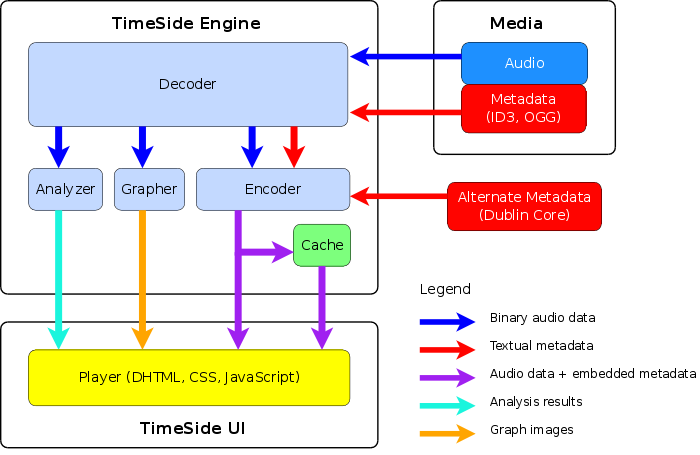
\includegraphics[width=\textwidth]{img/timeside_schema.png}
  \end{center}
\end{frame}
\begin{frame}\tiny
  \frametitle{Processors}
  \begin{minipage}{0.45\linewidth}

   \begin{block}{IDecoder}
      \begin{itemize}
      \item FileDecoder \texttt{[gst\_dec]}
      \item \alert{ArrayDecoder} \texttt{[array\_dec]}
      \end{itemize}
    \end{block}
    \begin{block}{IAnalyzer}
      \begin{itemize}
      \item Level \texttt{[level]}
      \item MeanDCShift \texttt{[mean\_dc\_shift]}
      \item AubioTemporal \texttt{[aubio\_temporal]}
      \item AubioPitch \texttt{[aubio\_pitch]}
      \item AubioMfcc \texttt{[aubio\_mfcc]}
        \item AubioMelEnergy \texttt{[aubio\_melenergy]}
      \item AubioSpecdesc \texttt{[aubio\_specdesc]}
      \item \alert{Yaafe} \texttt{[yaafe]}
      \item \alert{Spectrogram} \texttt{[spectrogram\_analyzer]}
      \item \alert{Waveform} \texttt{[waveform\_analyzer]}
      \item \alert{VampSimpleHost} \texttt{[vamp\_simple\_host]}
      \item \alert{IRITSpeechEntropy} \texttt{[irit\_speech\_entropy]}
      \item \alert{IRITSpeech4Hz} \texttt{[irit\_speech\_4hz]}
      \item \alert{OnsetDetectionFunction} \texttt{[odf]}
      \end{itemize}
    \end{block}
   \end{minipage} \hfill
   \begin{minipage}{0.5\linewidth}
      \begin{block}{IEncoder}
      \begin{itemize}
      \item VorbisEncoder \texttt{[gst\_vorbis\_enc]}
      \item WavEncoder \texttt{[gst\_wav\_enc]}
      \item Mp3Encoder \texttt{[gst\_mp3\_enc]}
      \item FlacEncoder \texttt{ [gst\_flac\_enc]}
      \item AacEncoder \texttt{[gst\_aac\_enc]}
      \item WebMEncoder \texttt{[gst\_webm\_enc]}
      \end{itemize}
    \end{block}
  \begin{block}{IGrapher}
      \begin{itemize}
      \item Waveform \texttt{[waveform\_simple]}
      \item WaveformCentroid \texttt{[waveform\_centroid]}
      \item \alert{WaveformTransparent} \texttt{[waveform\_transparent]}
      \item WaveformContourBlack \texttt{[waveform\_contour\_black]}
      \item WaveformContourWhite \texttt{[waveform\_contour\_white]}
      \item SpectrogramLog \texttt{[spectrogram\_log]}
      \item \alert{SpectrogramLinear} \texttt{[spectrogram\_linear]}
      \end{itemize}
    \end{block}
   \end{minipage}

\end{frame}
\begin{frame}
  \frametitle{Principales nouveautés}
  \begin{block}{}
    \begin{itemize}
    \item Version 0.5.2
    \item Mise en place d'une documentation :
      \url{http://files.parisson.com/timeside/doc/}
   
    \item Installation par paquets Debian (Timeside + Aubio + Yaafe)
      pour Debian Stable 7.0 Wheezy
      \url{https://github.com/yomguy/TimeSide\#install}
    \item Outil en \emph{ligne de commande} : \texttt{timeside-launch}
    \item Décodeur : possibilité de lire un \alert{segment} de fichier audio
    \end{itemize}
  \end{block}
  \begin{block}{Analyseurs - Sauvegarde des résultats}
    \begin{itemize}
    \item Amélioration de la sérialisation des resultats (xml, json,
      yaml, \alert{numpy}, \alert{hdf5})
    \item  Ajout de fonctionnalités et \emph{Réusinage} de code en prévision de l'intégration de méthodes d'analyse automatique
    \end{itemize}
    
  \end{block}
\end{frame}

\begin{frame}{Extraction de descripteurs audio}
  
 \begin{block}{Audio features extraction}
TimeSide incorpore des bibliothèques d'extraction de descripteurs audio de référence :
\vspace{-0.1cm}
\begin{itemize} \tiny
\item \textbf{Aubio:
    \colorbox{yellow!50}{\hskip1ex  \url{http://aubio.org} \hskip1ex }}
\vspace{-0.1cm}
\item \textbf{Yaafe:
    \colorbox{yellow!50}{\hskip1ex \url{http://yaafe.sourceforge.net}\hskip1ex }}
\vspace{-0.1cm}
\item \textbf{Vamp plugins:  
    \colorbox{yellow!50}{\hskip1ex \url{http://www.vamp-plugins.org}\hskip1ex }} 
\end{itemize}
\alert{A partir de ses descripteurs, les analyses automatiques pour chaque item d'une collection peuvent être mises en place}\\
$\longrightarrow$ Intégration des premiers analyseurs ``DIADEMS'' : Détecteurs de segments de paroles (IRIT) 

\end{block}
\begin{block}{}
  Formalisation de différents types de résultats :
      \begin{itemize}
      \item time\_mode : global, event, segment, framewise
      \item data\_mode : value, label
      \end{itemize}
\end{block}
\end{frame}

\begin{frame}[fragile]
  \begin{block}{TimeSide - Dépôt Github}
    \begin{center}\scriptsize
      \colorbox{yellow!50}{\bf \hskip3ex
        \url{https://github.com/yomguy/TimeSide/} \hskip3ex }
    \end{center}
3 branches principales :
  \begin{itemize}
  \item master (0.5.2)
  \item dev
  \item \alert{diadems} $\longleftarrow$ \emph{vos précieuses contributions}
  \end{itemize}
  \end{block}
  \begin{block}{Installation}
\url{https://github.com/yomguy/TimeSide\#install}
    \begin{itemize}
    \item Installation des dépendances :
\begin{lstlisting}[language=bash, basicstyle=\TINY]
$ echo "deb http://debian.parisson.com/debian/ stable main" |
$ sudo tee -a /etc/apt/sources.list 
$ echo "deb-src http://debian.parisson.com/debian/ stable main" | sudo tee -a /etc/apt/sources.list 
$ sudo apt-get update 
$ sudo apt-get install git 
$ sudo apt-get build-dep python-timeside
\end{lstlisting}

    \item Installation depuis le dépôt \emph{Github} :
\begin{lstlisting}[language=bash, basicstyle=\TINY]
$ git clone https://github.com/yomguy/TimeSide.git 
$ cd TimeSide 
$ git checkout dev 
$ export PYTHONPATH=$PYTHONPATH:`pwd` 
$ python tests/run_all_tests
\end{lstlisting}
\end{itemize}
\end{block}
\end{frame}

\begin{frame}[fragile]
  \begin{block}{Code Example (Python)}
    \vskip1ex
     \begin{minipage}{0.6\linewidth}
       \begin{lstlisting}
import timeside

# Define some processors:
decoder = timeside.decoder.FileDecoder('sweep.wav')

analyzer = timeside.analyzer.Level()
irit4hz = timeside.analyzer.IRITSpeech4Hz()

grapher = timeside.grapher.Spectrogram()
encoder = timeside.encoder.VorbisEncoder('sweep.ogg')

# Then, the magic pipeline:
(decoder | analyzer | irit4hz | grapher | encoder).run()

# Get the results:
grapher.render(output='image.png')
for key in analyzer.results.keys():
    print '%s in %s : %s'% (analyzer.results[key].name,
                            analyzer.results[key].unit,
                            analyzer.results[key].data)
 \end{lstlisting}
     \end{minipage}
    \hskip2ex
    \begin{minipage}{0.32\linewidth}
      \begin{center}
        \textbf{Results}
        \begin{figure}
          \centering
          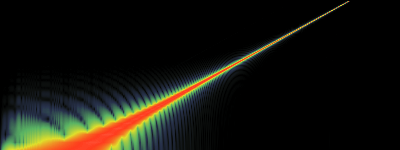
\includegraphics[width=\linewidth]{img/spectrogram.png}
          \caption{Spectrogram (sweep signal)}
        \end{figure}
      \end{center} 
      \vskip5ex
      \begin{lstlisting}
        Level Analyzer Max:[-6.021] 
        Level Analyzer RMS:[-9.856]
      \end{lstlisting}
 \end{minipage}
  \end{block}
\end{frame}

\begin{frame}
\frametitle{Détecteur de parole IRIT (4Hz modulation)}
\begin{center}
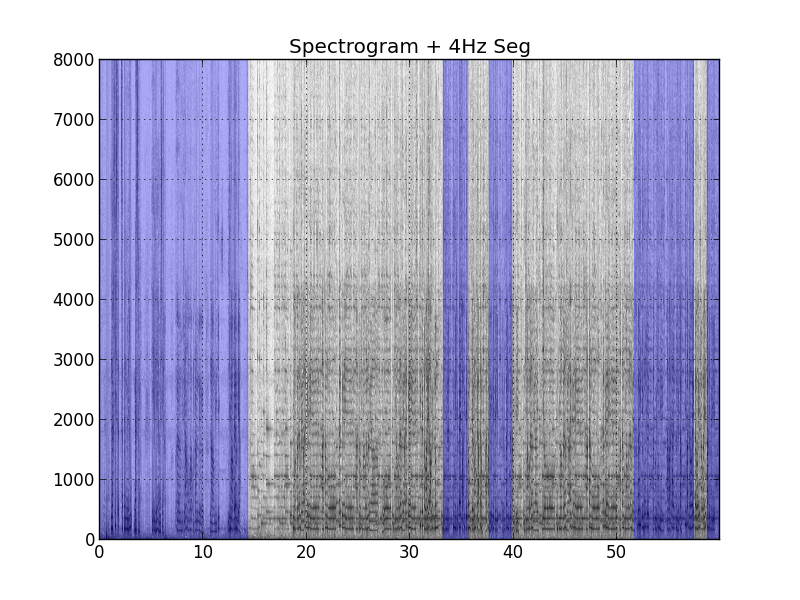
\includegraphics[width=0.8\linewidth]{img/irit_speech4hz}\\
\href{sounds/CNRSMH_I_2013_202_001_06.mp3}{Son}
\end{center}
\end{frame}
\begin{frame}\frametitle{Aubio Pitch + Aubio Beat}
  \begin{center}
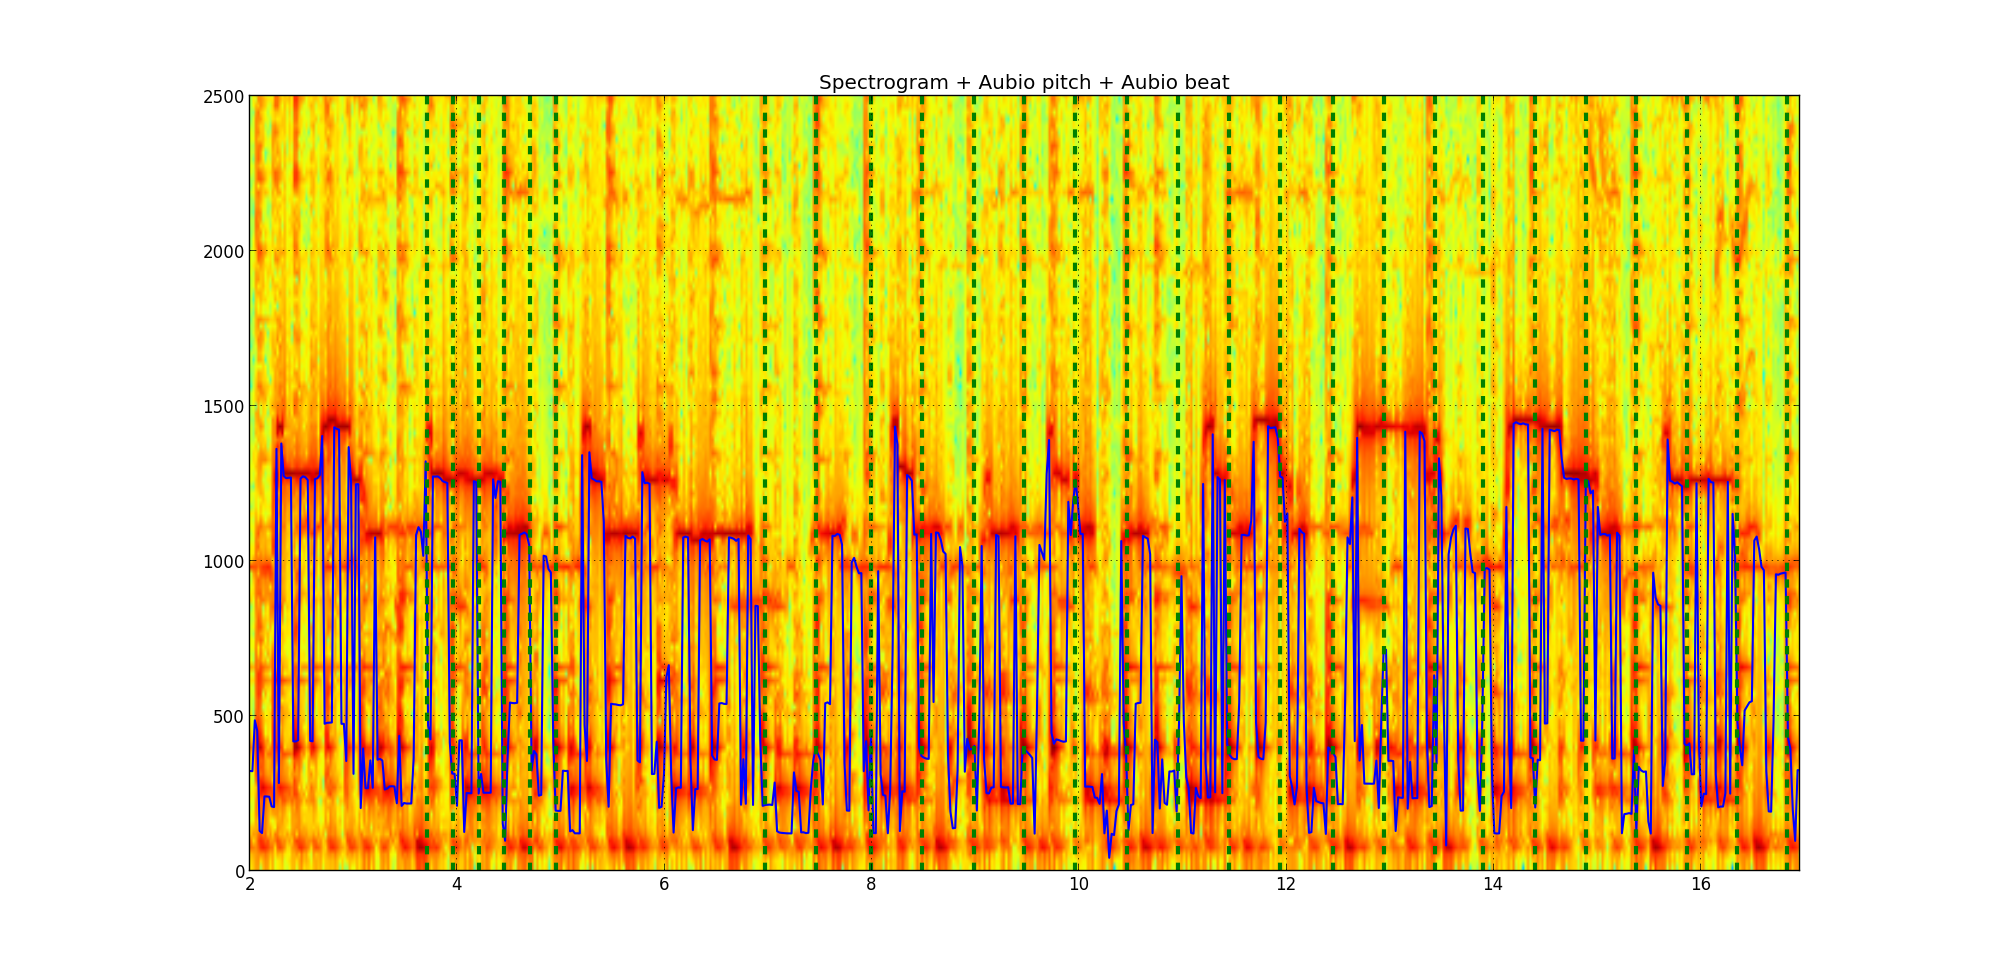
\includegraphics[width=1.1\linewidth]{img/aubio_pitch_beat.png}\\
\href{sounds/CNRSMH_E_1985_001_001_001_04.mp3}{Son}
\end{center}
\end{frame}
\end{document}
%%% Local Variables: 
%%% mode: latex
%%% TeX-master: t
%%% End: 
